% se volete aggiungere figure sintassi:
% \begin{figure}[htbp]
% [\centering]
% \includegraphics[height=,width=[\textwidth],scale=,angle=]{PATH}
% \caption{descrizione della figura[\label{figure:label}]}
% \end{figure}
% comunque è da vedere il risultato e eventualmente adattarlo

% CLASSE DEL DOCUMENTO
\documentclass[a4paper,11pt]{report}

% PREAMBOLO

% per gestione lingua e caratteri
\usepackage[italian]{babel}
\usepackage[utf8x]{inputenc}
\usepackage[T1]{fontenc}

% per gestione figure
\usepackage{graphicx}
\usepackage{float}

\frenchspacing

% valori che modificano il titolo
\title{Social-Wireless}
\author{Andrei Palamarciuc matr. 784068 \\ Stefano Bielli matr. 804253 \\ Luca Borghese matr. 800606}
\date{03/03/2014}

% INIZIA IL DOCUMENTO
\begin{document}

\maketitle
\tableofcontents
%\listoffigures
%\listoftables

\chapter{Introduzione}
Questo progetto si propone di far apprendere agli studenti tecnologie rivolte verso i sistemi embedded. Attraverso l’uso della board STM32F4 DISCOVERY, fornita da STMicroelectronics, il sistema operativo real-time Miosix, sviluppato internamente al politecnico di Milano da Terraneo Federico, e il modulo wireless nRF24L01, prodotto dalla NORDIC SEMICONDUTOR, andremo a sviluppare un software in grado di trasmettere pacchetti di dati tramite il collegamento wireless tra due board. Inoltre ci sarà un’integrazione del software con due altri gruppi di progetto che si sono occupati, in ordine, di utilizzare l’accelerometro, in modo tale da creare un pedometro, e della riproduzione vocale.

\chapter{Strumenti usati}

\section{Board STM32F4}
Per lo sviluppo dell'applicazione è stato usato il microcontrollore STM32F407VG\cite{manual-stm32f4} fornito dall'azienda STMicroelectronics\cite{stm}. Questo microcontrollore è fornito di un numero elevato di periferiche e GPIO, ottimo per lo sviluppo di applicazioni abbastanza articolate. La documentazione inoltre è risultata affidabile e completa.\par

\subsection{Interrupt EXTI1}
La periferica EXTI1 è stata utilizzata poiché il modulo wireless, con cui ci interfacciamo, scatena un interrupt quando riceve un nuovo pacchetto o quando trasmette un pacchetto. Quindi il pin di interrupt del modulo nRF24L è collegato via gpio alla periferica EXTI1 che viene configurata in modo tale da scatenare un interrupt interno.

\subsection{Periferica SPI}
La periferica SPI della board è configurabile attraverso due registri interni, il control register 1 e il control register 2; con questi due registri è possibile modificare il comportamento della periferica per adattarlo alla variante di protocollo dei dispositivi a cui è collegato.
Inoltre è possibile controllare lo stato della periferica attraverso lo status register. Con questi tre registri è possibile controllare completamente la periferica per ricevere e inviare dati utilizzando il protocollo spi.\par
Per l'invio e la ricezione dei dati è possibile utilizzare due registri che fanno riferimento entrambi al nome data register, cioè con riferimento alla fig. \ref{figure:diagramma_spi} in lettura si legge Rx Buffer e in scrittura si scrive su Tx Buffer. Per approfondimento si richiama il reference manual della board\cite{manual-stm32f4}.
\begin{figure}[H]
	\centering
	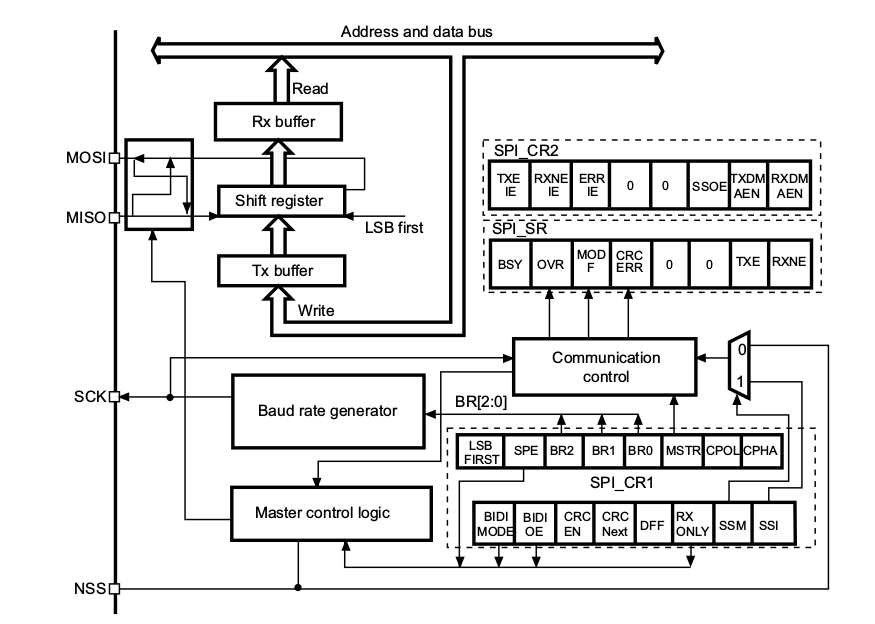
\includegraphics[width=\textwidth]{figure/diagramma_spi.png}
	\caption{Periferica SPI della Board STM32F4\label{figure:diagramma_spi}}
\end{figure}

\section{Modulo wireless nRF24L01}
Per implementare la funzionalità wireless, cioè la possibilità di trasmettere dati da una board all'altra, è stato utilizzato
il modulo MOD-NRF24LR della Olimex, che unisce attraverso un PCB il circuito integrato NRF24L01 all'elettronica necessaria
al suo funzionamento (condensatori, induttori, antenna, oscillatore e supporto fisico).\par
\begin{figure}[H]
	\centering
	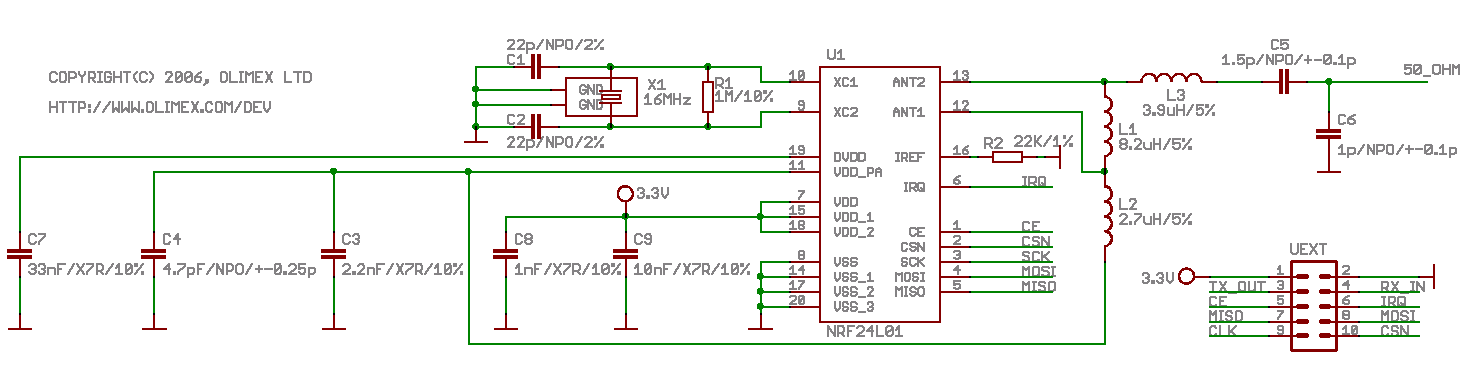
\includegraphics[width=1.0\textwidth]{figure/MOD-NRF24L-ELECTRICAL.png}
	\caption{MOD-NRF24LR: Circuito}
\end{figure}
NRF24L01 si interfaccia attraverso 6 pin: 4 pin per la periferica SPI (CSN, SCK, MOSI, MISO), chip enable (CE) e interrupt (IRQ).
Attraverso questi è possibile configurare la modalità di funzionamento e accedere a tutte le funzionalità.\par
Le caratteristiche principali del modulo wireless:
\begin{itemize}
	\item 2.4GHz ISM;
	\item Velocità di trasmissione: 1Mbps o 2Mbps;
	\item Enhanced ShockBurst™: payload dinamico;
	\item Potenza trasmissione: 0, -6, -12 o -18dBm;
	\item Sensitività ricezione: -82dBm.
\end{itemize}
Il funzionamento di NRF24L01 è rappresentato dalla macchina a stati in fig. \ref{figure:macchina_a_stati}.
Per spostarsi da uno stato ad un'altro è necessario cambiare il valore di alcuni registri e/o agendo sulla linea CE. I registri del modulo sono scrivibili utilizzando opportuni comandi\footnote{ un comando è un insieme di 1 o più byte} inviati attraverso la periferica SPI.\par
Il lavoro fatto è stato quello di implementare una macchina a stati (lato microcontrollore) che gestisce la macchina a stati di NRF24L01.
\begin{figure}[H]
	\centering
	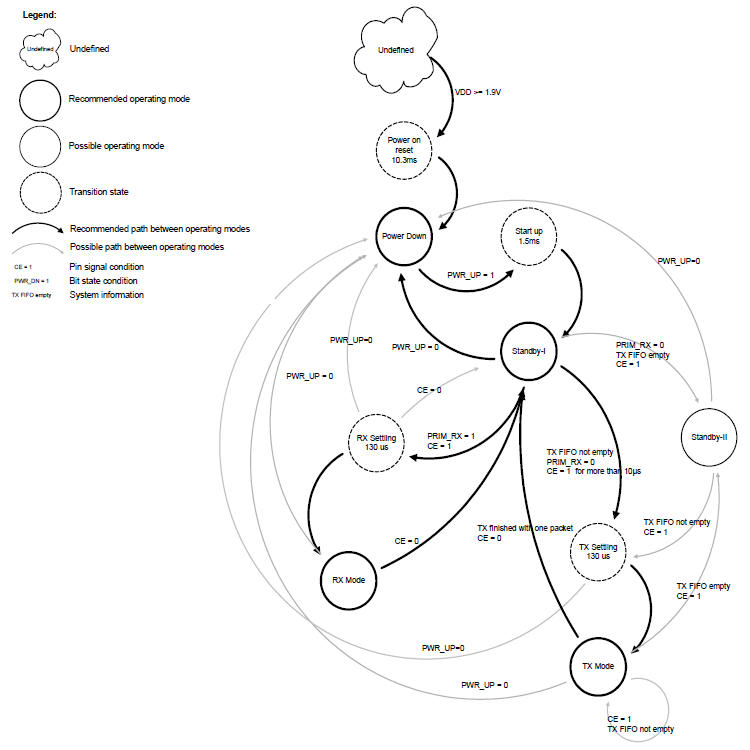
\includegraphics[width=1.0\textwidth]{figure/nrf-state-diagram.png}
	\caption{NRF24L01: Macchina a stati\label{figure:macchina_a_stati}}
\end{figure}

\section{Miosix}
Miosix\cite{miosix} è un sistema operativo real-time sviluppato dal Dottorando del Politecnico di Milano Terraneo Federico, distribuito sotto i termini della GNU Public License\cite{gnu-license} della Free Software Foundation\cite{free-software-foundation}. Peculiarità di questo sistema operativo è la completa scrittura in linguaggio c++ e un'offerta di API posix per utilizzo di thread.\par
L'utilizzo del linguaggio c++ ha portato a una grande affidabilità del sistema, riscontrata anche dal gruppo durante i test del progetto, e a una facile estensibilità, sia del sistema stesso sia per lo sviluppo di applicazioni; quest'ultima agevolata ulteriormente dall'offerta di API standard oramai affermate e uno sviluppo del sistema costante per adattarlo alle novità tecnologiche.

\section{Git}
Per quanto riguarda la sincronizzazione tra i componenti del gruppo e la condivisione del codice è stato usato git\cite{git}, un source control manager distribuito. Per far questo sono stati usati due repository on-line serviti dai siti bitbucket e github; il primo è stato usato solo dai componenti del gruppo, il secondo è stato fornito dai professori per la consegna. Il ramo usato dal gruppo nel repository della consegna si chiama grp63.
\begin{figure}[htbp]
	\centering
	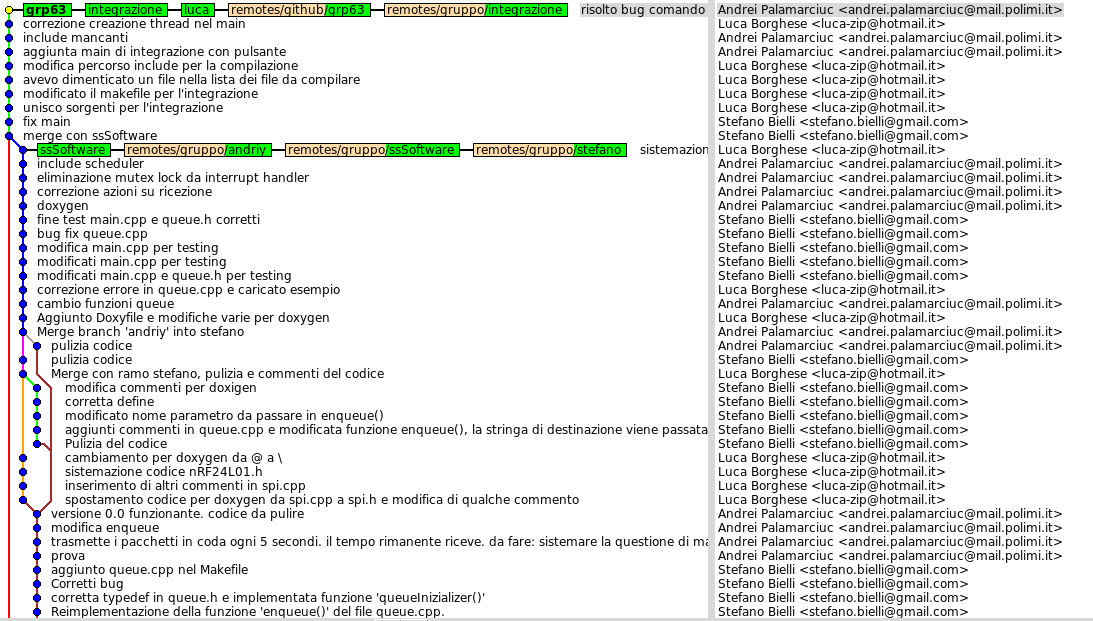
\includegraphics[width=\textwidth]{figure/git.png}
	\caption{Esempio di commit eseguiti dal gruppo\label{figure:git}}
\end{figure}

\chapter{Codice}
Il codice è stato separato in tre blocchi sia per una divisione funzionale sia per dividerlo tra i membri del gruppo:
\begin{enumerate}
	\item Uso della periferica spi\cite[spi.cpp]{social-wireless};
	\item Gestione di una coda di invio\cite[queue.cpp]{social-wireless};
	\item Configurazione e l'uso del modulo wireless\cite[social-wireless.cpp]{social-wireless}; include una parte di routine di risposta ad un interrupt;
\end{enumerate}

\section{Codice Interrupt}
Quando si riceve l'interrupt dal modulo nRF24L(che scatena poi un interrupt della periferica EXTI1) parte la routine di risposta all'interrupt:
\begin{verbatim}
void __attribute__((used)) EXTI1HandlerImpl(){
    
    EXTI->PR = EXTI_PR_PR1;   
    
    if(waiting==0) return;
    waiting->IRQwakeup();
    if(waiting->IRQgetPriority()>Thread::IRQgetCurrentThread()->IRQgetPriority()) 
    	Scheduler::IRQfindNextThread();
    waiting=0;
     
    greenLed::high();
}
\end{verbatim}
la routine di interrept controlla se esiste un thread in attesa di quell'evento e se è così lo sveglia.

\section{Codice Spi}
Il codice della periferica spi si divide sostanzialmente in due parti:
\begin{enumerate}
	\item Configurazione della periferica spi2 per la comunicazione con il modulo nRF24L;
	\item Uso della periferica(invio o ricezione dei dati).
\end{enumerate}
Nella parte di configurazione viene abilitato il clock alle parti della board usate per la comunicazione, vengono scritti i registri control register 1 e control register 2 per adattare il comportamento della periferica alla comunicazione con il modulo wireless nRF24L.\par 
Per quanto riguarda l'invio e la ricezione dei dati sono state implementate due funzioni, fatte appositamente per la comunicazione con il modulo wireless, una di invio e una di ricezione dati.
A queste funzioni va passato un comando da inviare per primo che farà capire al modulo cosa vogliamo fare e poi, a seconda della funzione(di invio o ricezione), si procede alla comunicazione.

\section{Codice coda}
Si è pensato di utilizzare una coda per risolvere i problemi dovuti a possibili conflitti dovuti a chiamate di invio dati concorrenti.
Tale coda è stata implementata come una semplice coda circolare di tipo FIFO e grandezza di 1024 Byte.
Vengono fornite quattro funzionalità di base per l’utilizzo:
\begin{description}
	\item [void queueInizializer(queue\_t* queue)] si occupa della inizializzazione di un nuovo dato di tipo coda;
	\item [int queuePush(char* data, queue\_t* queue)] fa un push di dati nella coda;
	\item [void queuePop(queue\_t* queue, char* dest)] fa un pop di dati dalla coda;
	\item [bool queueIsEmpty(queue\_t* queue)] controlla se ci sono elementi nella coda.
\end{description}

\section{Codice inizializzazione modulo wireless}
Questa parte di codice imposta la modalità di funzionamento di NRF24L01: i registri vengono scritti con opportuni valori che impostano
la velocità di trasmissione, tipo di payload, indirizzo di trasmissione e di ricezione, ecc. Di seguito è mostrato il diagramma di flusso del
codice:
\begin{figure}[H]
	\centering
	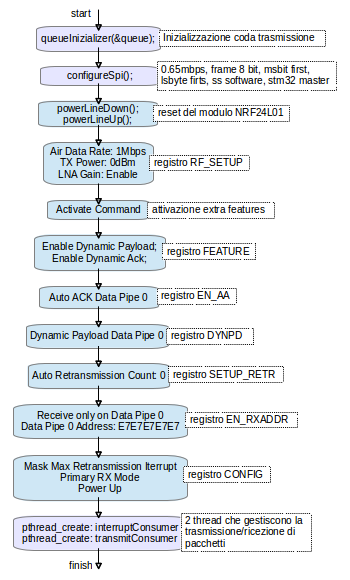
\includegraphics[width=.6\textwidth]{figure/init-wireless.png}
	\caption{social\_wireless.cpp: funzione socialWirelessInit()}
\end{figure}

\section{API fornita}
L'API fornita dal gruppo consiste in due funzioni:
\begin{description}
	\item [socialWirelessInit()] Funzione che crea i due thread usati per la comunicazione e inizializza tutte le periferiche;
	\item [int socialWirelessSendData(char* payload)] Funzione che riempie la coda di invio per trasmettere dei dati. 
\end{description}
comunque per dettagli vedere la documentazione del codice\cite{social-wireless}.

\chapter{Sincronizzazione tra task}
La trasmissione di un pacchetto attraverso il canale radio richiede qualche ms e per evitare di bloccare così a lungo la funzione \emph{socialWirelessSendData(char* payload)} offerta dall'interfaccia si è fatto uso di una coda e di un thread\footnote{transmitConsumer} che si sveglia ogni 50ms e trasmette un pacchetto dalla coda. Anche per ricevere un pacchetto si è fatto uso di un thread\footnote{interruptConsumer}, che si differenzia dal precedente per il fatto che viene svegliato dalla routine di interrupt e non in modo periodico.\par
Avendo due thread concorrenti che condividono le stesse risorse (coda e modulo NRF24L01) è stato necessario sincronizzarli. Di seguito sono mostrati i flussi di esecuzione dei thread e delle funzioni \emph{socialWirelessSendData(char* payload)} e \emph{EXTI1HandlerImpl}.
\begin{figure}[H]
	\centering
	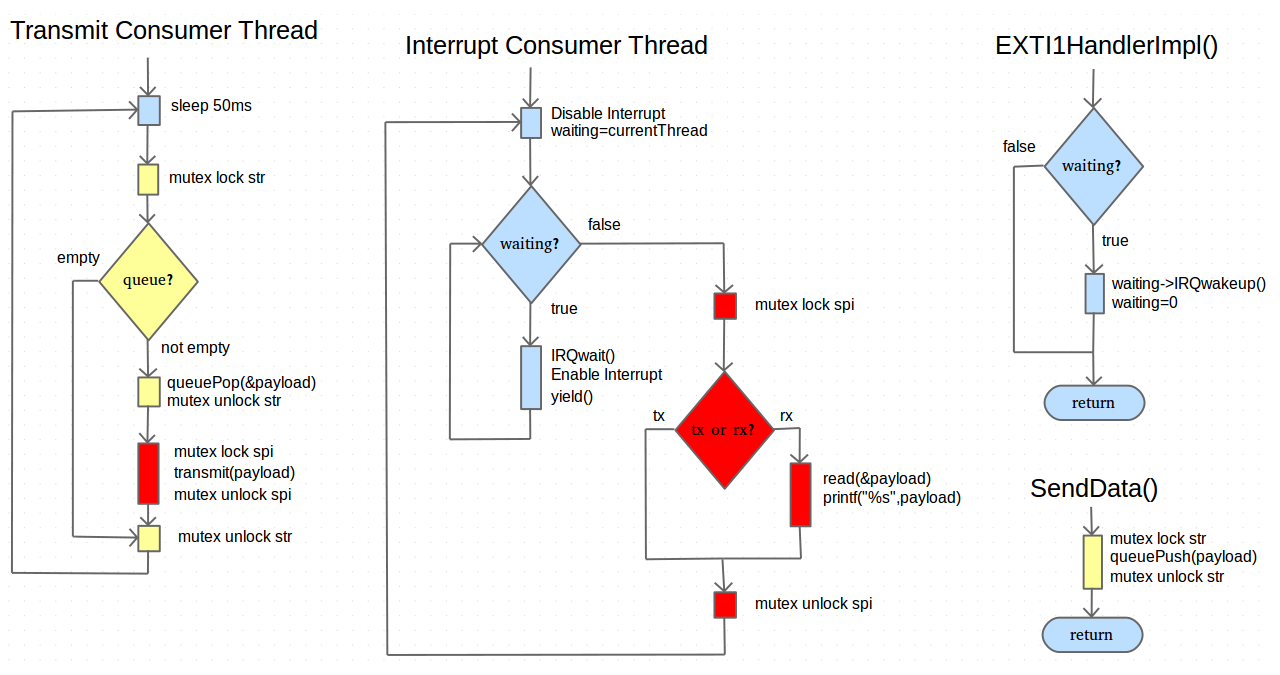
\includegraphics[width=1\textwidth]{figure/thread-sinc-v2.png}
	\caption{Sincronizzazione tra task}
\end{figure}

\chapter{Integrazione}
L'integrazione è stata fatta con due moduli che abbiamo reputato più interessanti per le funzionalità offerte e sono i gruppi 31(sonoro) e 13(pedometro). C'è da dire che l'integrazione con solo questi gruppi è stata forzata dai diversi tempi di sviluppo tra i vari gruppi, cioè la maggior parte degli altri gruppi non disponevano di un api adatta al momento del nostro interessamento.

\section{Gruppo pedometro}
Il gruppo 13 del pedometro è composto dagli studenti Diego Rondelli e . Il codice di questo gruppo fornisce un oggetto pedometro, con un design pattern di generazione singleton, che fornisce questa interfaccia pubblica:
\begin{verbatim}
class Pedometer
{
public:

static Pedometer* getInstance();
void start();
int getStep();
void compareSteps(int otherSteps);
\end{verbatim}
la funzione start inizia il conteggio dei passi, getSteps ritorna il numero di passi fatti dall'utente e compareSteps compara il numero di passi fatti dall'utente con l'intero otherSteps e utilizza il codice del gruppo audio per dare un riscontro audio all'utente.
Noi utilizziamo questa API trasmettendo il numero di passi ottenuto con getSteps via wireless alla pressione del bottone della board, e quando la board riceve un intero chiama la funzione compareSteps per un riscontro audio dello stato.

\section{Gruppo sonoro}
Il gruppo 31 sonoro è composto da Marco Mezzanotte, Tommaso Calcina e . Non abbiamo utilizzato direttamente il loro codice in quanto il codice del pedometro integra l'uso di questa parte. A grandi linee il gruppo fornisce un oggetto ring, creato con design pattern singleton, e fornisce un'interfaccia pubblica:
\begin{verbatim}
class ring {
public:

static ring& instance();
void play_n_of_step(int steps,int volume);
void looser_Song(int volume);
void victory_Song(int volume);
\end{verbatim}
Analizziamo le varie funzioni:
\begin{description}
	\item [instance] fornisce l'oggetto ring;
	\item [play\_n\_of\_step] riproduce il numero di passi \emph{steps} con volume \emph{volume};
	\item [looser\_Song] riproduce un motivo di sconfitta con volume \emph{volume};
	\item [victory\_Song] riproduce un motivo di vittoria con volume \emph{volume}.
\end{description}

\chapter{Conclusione}
Il progetto ha permesso a tutti i membri del gruppo di acquisire conoscenze in campi mai visti in altri corsi universitari e affrontare problemi mai incontrati in altri progetti. In particolare abbiamo acquisito conoscenze approfondite del processo di compilazione, una preparazione sufficiente per la lettura dei datasheet, una discreta conoscenza degli standard per la programmazione con board di prototipazione e l'uso di sistemi operativi real-time per semplificare la programmazione multi-tasking.\par
I principali problemi affrontati dal gruppo sono stati per lo più teorici, è stato grande il lavoro iniziale per lo studio degli strumenti hardware utilizzati e i protocolli utilizzati da questi per la comunicazione. Per quanto riguarda la programmazione, una buona divisione iniziale dei compiti ha permesso uno sviluppo abbastanza veloce della parte software del progetto e l'uso di git è stato estremamente utile per la sincronizzazione tra i vari membri e anche per la parte di integrazione finale. Inoltre in quest'ultima parte il buon stile di programmazione attuato dagli altri due gruppi ha permesso un'integrazione molto veloce e senza errori, grazie anche all'uso di Miosix e del linguaggio c++.\par
Unica pecca del progetto è stata la bassa comunicazione tra i vari gruppi e la conseguente scarsa integrazione; forse si sarebbe potuto migliorare questo aspetto con una partecipazione obbligatoria a degli incontri in università per la discussione di questo, in quanto non ci sono state iniziative da parte degli studenti.

\begin{thebibliography}{99}

	\bibitem{manual-stm32f4} stm microcontroller catalog web site,\\http://www.st.com/web/en/catalog/mmc/SC1169/SS1577/LN11
	\bibitem{stm} st official web site, http://www.st.com/
	\bibitem{miosix} Miosix official site, http://www.miosix.org/
	\bibitem{gnu-license} gnu official web site, http://www.gnu.org/
	\bibitem{free-software-foundation} Free Software Foundation official site, http://www.fsf.org/
	\bibitem{git} Git official site, http://www.git-scm.com/
	\bibitem{social-wireless} Documentazione progetto Social-Wireless

\end{thebibliography}

\end{document}
